\providecommand{\main}{../..}%define path to bib for subfiles
\documentclass[../../main.tex]{subfiles}
\begin{document}
\onlyinsubfile{\setcounter{chapter}{8}}
\notinsubfile{}
\chapter{Experimenten}
\onlyinsubfile{
\marginpar{\vspace{0cm}
\textcolor{red}{ hoofdstuk is los gecompileerd, hstk nummer is 1}}
}
In een quantum computer gebruiken we verschijnselen als \textit{superpositie}, \textit{interferentie}, \textit{verstrengeling} en \textit{coherentie}. Dit zijn verschijnselen afkomstig uit de quantumfysica. Deze eigenschappen zijn essenetieel voor de werking van een quantumcomputer. In dit hoofdstuk verkennen we deze begrippen. We maken gebruik van natuurkundige principes ondersteund met enkele eenvoudige experimenten. We gebruiken hiervoor de eigenschappen van licht.

\section{Natuurkundige principes}

\subsection{Golf of deeltje}
Licht heeft eigenschappen van zowel golven als deeltjes. Twee eigenschappen die elkaar lijken uit te sluiten. Newton zag dat licht terugkaatste van een spiegel, en dat licht door een gaatje rechtdoor ging zoals een kogel dat doet. Huygens zag dat licht zich juist in alle richtingen kon voortplanten, zoals je een steen in de vijver gooit, een golfeigenschap. In het begin van de negentiende eeuw leek Thomas Young (1802) het pleit te beslechten door de inwerking van lichtbronnen op elkaar onderzoeken. Zij vertonen interferentie, een golfeigenschap. Op zijn experimenten gaan we dieper in. In de negentiende eeuw liet Maxwell zien dat licht een elektromagnetisch golfverschijnsel was. Deze golven zijn te polariseren, een eigenschap die licht ook vertoond. In 1905 toonde Einstein aan dat licht uit losse een energiepakketjes bestond, later fotonen genoemd. In de quantummechanica gebruiken we deeltjes- en golfeigenschappen al naar gelang.

\subsection*{Golven}
Anders dan deeltjes kunnen golven elkaar kruisen zonder te botsen. Denk maar eens wat er gebeurt als je twee waterstralen kruist of aan de kringen die regenruppels in een plas maken of als je twee lichtbundels kruist. 
\marginpar{\vspace{0cm}
\label{regen} \hrefnote{https://nl.depositphotos.com/107549482/stock-video-rain-drops-on-the-water.html}{regen}
}

In onze experimenten gebruiken we geluid en licht als golfverschijnsel. Er is wel een wezenlijk verschil tussen de manier waarop licht en geluid zich voortplanten.

\subsubsection{transversaal}
Als je een steen in de vijver gooit plant zich een rimpeling voort over het oppervlak van het water. De watermolekulen zelf bewegen niet in de voortplantingsrichting. Ze bewegen alleen op en neer op hun plaats. Dit is te zien als de golf een eendje passeert. Het eendje gaat alleen op en neer. Het beweegt loodrecht op de voortplantingsrichting.
\marginpar{\vspace{0cm}
Bij een \textit{transversale} golf staat de uitwijking loodrecht op de voortplantingsrichting van de golf. 
}

\subsubsection{longitudinaal}
Geluid is ook een golfverschijnsel maar de voortplanting van geluid vindt plaats door het botsen van luchtmoleculen in de richting van de voortplanting van de golf. We noemen dit \textit{longitudinaal}.
\marginpar{\vspace{0cm}
Bij een \textit{longitudinale} golf is de uitwijking van de trilling in de voortplantingsrichting van de golf.
}

\easy Is een wave in een stadion een longitudinale of een transversale golf?
\subsubsection*{polarisatie}
Licht is een transversale ruimtelijke golf met een uitwijking die in \textit{twee} richtingen loodrecht op de voortplanting van de golf kan staan. Licht kan gedwongen worden in juist een verticale of een horizontale richting te trillen.  
\marginpar{\vspace{0cm}
\hrefnote{https://www.youtube.com/watch?v=MzRCDLre1b4}{3blue1brown} geeft mooi grafisch weer hoe licht als zich electromagnetische golf voortplant.}
Deze eigenschap gebruiken we voor het experiment.
Geluid is niet polariseerbaar omdat het alleen in de voortplantingsrichting trilt. Een deel van de experimenten zijn daarom niet met geluid uit te voeren.

\subsection*{Interferentie}
De eigenschap dat golven door elkaar heen kunnen lopen geldt zowel voor longitudinale als voor transversale golven. We kunnen zowel geluid als licht gebruiken om dit verschijnsel te laten zien.

Een golf is een herhalend patroon. Bij het eendje op de watergolf komt er afwisselend een berg en een dal voorbij. Bij geluid passeert er afwisselend een drukverhoging en een drukverlaging (hoe vaker hoe hoger de toon). 

\subsubsection{Rowili}
Rowili is politie jargon voor het lint dat gebruikt wordt om afzettingen te maken. (rood-wit lint). 
met rowili kun je makkelijk interferentie van golven nabootsen. De witte stukken zijn de golftoppen, de rode de dalen. 
Als golven uit twee bronnen elkaar \textit{in fase} tegen komen (op het kruispunt van twee stukken lint) versterken ze elkaar. Van beide bronnen komen dan telkens tegelijk bergen en dalen. Als ze in \textit{tegenfase} staan doven ze elkaar juist uit. Een top (wit stuk) wordt opgeheven door een dal (rood) uit de andere kant en een halve trilling later werkt het andersom, maar dan doven zij elkaar weer uit.
\marginpar{\vspace{0cm}
\textit{coherentie} twee of meer bronnen met dezelfde frequentie zijn coherent. Het fase verschil is dan constant en kan nul zijn.
}
Voor interferentie is het nodig dat de bronnen\textit{ coherent} zijn.

\marginpar{
De \textit{fase} van een trillingsbron is het aantal trillingen dat de bron heeft uitgevoerd. We zijn meestal alleen ge\"interesseerd in de fractie van een trilling. Een fase van \si{0,25} betekent dat de trilling een kwart van zijn beweging heeft uitgevoerd.
}


\vspace*{.5\baselineskip plus 2pt}
\noindent\begin{tikzpicture}
\node [extra] (box){%
\begin{minipage}{\dimexpr\linewidth-2\fboxrule-2\fboxsep\relax}
Twee geluidsbron met een toon van ongeveer \SI{1}{\kilo\hertz}. Doe een vinger in je oor en ga met je hoofd langzaam heen en weer. Je zult op sommige plekken extra hard geluid, en op sommige plekken nagenoeg stilte ervaren. De stille plekken noemen we knopen, de extra luide plekken heten buiken. Merk op, deze plekken bewegen niet met de golf mee, ze staan op vaste plekken in de ruimte. Dit verschijnsel noemen we interferentie.

Zoek de voortplantingssnelheid van geluid op.

\end{minipage}
};
\node[extratitle] at (box.north west) {Experiment};
\end{tikzpicture}%
%


\subsection*{Knopen en buiken}
Als twee stukken lint bij elkaar komen en er komen uit beide richtingen tegelijk bergen en dalen aan, in \textit{fase}, dan is de uitwijking op die plaatsen extra heftig: hard geluid, veel licht. We noemne zo'n plek een \textit{buik}. Als er van een bron juist een dal komt en van uit de andere juist en berg, dan zijn de bronnen in \textit{tegenfase}.  Ze heffen elkaar op. We noemen zo'n plek een een \textit{knoop}.
De golfbergen en dalen bewegen in de ruimte met de snelheid van de golf, maar de buiken en knopen staan op vaste plaatsen.
We voerden de experimenten met interferentie van geluid uit met \'e\'en toonhoogte. Bij andere golflengten liggen de knopen en buiken op andere plaatsen. Als je ze door elkaar gebruikt zoals bij muziek merk je er niets meer van.
\easy{Je kunt geluidsgolven niet polariseren. Waarom niet?}

\subsection*{\easy laser}
Laserlicht heeft \'e\'en kleur, \'e\'en golflengte. Dit licht is dus heel goed te gebruiken als coherente lichtbron voor interferentie experimenten. Het is ook nog eens heel intens, dat is handig.
 
\subsection*{Enkelspleet}
Licht dat door een smalle spleet gaat (kleiner dan de golflengte) waaiert uit als een halve cirkel. Als de spleet breder wordt (in ons experiment tot zo'n 200 golflengten) verandert dit patroon. In de richting loodrecht op de spleet zijn alle punten in fase, maar in een willekeurige scheve richting treedt  er een fase verschil op. Er onstaan donkere vlekken op het scherm.

\subsection*{Dubbelspleet}
Met twee spleten vlak naast elkaar hebben we het experiment van Young nagebouwd. Hij zag dat de golven na de dubbelspleet interfereerden. Wij trekken het experiment van Young door naar de 19e eeuw door het uit te breiden met polarisatie.

\subsection*{Polarisatie}
\marginpar{\vspace{-4cm}
polarisatie vonkenopstelling Urs
}
Je kunt licht voorstellen als een transversale golf die zich met de lichtsnelheid voortbeweegt. De amplitude van de transversale beweging is twee dimensionaal voor te stellen als een roterende vector. De lichtvector plant zich zo als een kurkentrekker beweging voort. Lineaire polarisatiefilters projecteren deze ronddraaiende beweging op een as, daarmee wordt de beweging een trilling in \'e\'en richting. Laten we die richting vertikaal noemen.
\marginpar{\vspace{-5cm}
\begin{tikzpicture}[scale=.45,domain=-1:7, samples=100]
\draw[help lines,color=gray] (-1.1,-1.1) grid (7.1,7.1);
\draw[] (0,-1.2) -- (0,7.2) node[above] {$Y$};
\draw[] (-1.2,0) -- (7.2,0) node[below] {$X$};
\draw [black, thick, ->, >=triangle 45] (0,0) --(0,6);
\draw [green, thick, ->, >=triangle 45] (0,0)-- (45:4.24);
\draw [black, thick, dashed] (0,6) -- (45:4.24);
\draw [black, thick, dashed] (45:4.24) -- (3,0);
\draw [red,   thick, ->, >=triangle 45] (0,0) --(3,0);
\end{tikzpicture}
\captionof{figure}{projecties\label{fig:projecties}}
} 
Als we een tweede filter hierachter zetten, in dezelfde richting, wordt het licht nog wel iets verzwakt vanwege de plastic film. Als we het tweede filter draaien komt er steeds minder licht door, tot het licht bij \SI{90}{\degree} volledig geblokkeerd wordt. In fig.~\ref{fig:maluslaw}staat de doorgelaten intensiteit als functie van de draaiingshoek van het tweede filter getekend.
\marginpar{\vspace{0cm}
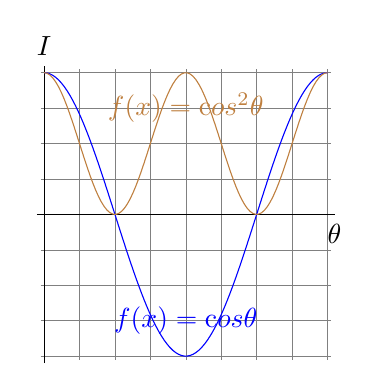
\begin{tikzpicture}[scale=.45,domain=0:8, samples=100]
\draw[very thin,color=gray] (-0.1,-4.1) grid (8.1,4.1);
\draw[] (-0.2,0) -- (8.2,0) node[below] {$\theta$};
\draw[] (0,-4.2) -- (0,4.2) node[above] {$I$};
\draw[color=blue] plot (\x,{4*(cos{(\x*45)})});
\node[color=blue] at (4,-3) {$f(x) = \mathrm cos{\theta}$};
\draw[color=brown] plot (\x,{4*(cos{(\x*45)})^2});
\node[color=brown] at (4, 3) {$f(x) =  \mathrm cos^{2}{\theta}$};
\end{tikzpicture}
\captionof{figure}{wet van Malus\label{fig:maluslaw}}
} 

Wat gebeurt er als je een derde filter onder een hoek van \SI{45}{\degree} \textit{tussen} twee loodrechte polaroids plaatst? Het licht keert weer terug!
In figuur~\ref{fig:projecties} staat het uitgetekend. Als we twee keer na elkaar een filter onder een hoek van \SI{45}{\degree} toepassen op vertikaal gepolariseerd licht eindigen we ook met horizontaal gepolariseerd licht, maar nu houden we wel licht over.
Hint $\mathrm{cos~\SI{45}{\degree}  =\tfrac{1}{\sqrt{2}}}$.
Twee keer toegepast wordt de amplitude dus gehalveerd, De energie wordt dus een vierde (niet meegenomen is verlies als gevolg van  de grijswaarde van de plastic drager).

Onze ogen meten net als iedere sensor de intensiteit. De 
polarisatiefilters projecteren de echter de amplitude. Net als bij een gewone trilling is de energie evenredig met het kwadraat van de amplitude.
\easy Zoek de grootheid intensiteit op. In welke SI eenheden druk je die uit?
\diff Iemand plaatst twee  filters tussen de orthogonale polarisers, telkens onder een hok van \SI{30}{\degree} ten opzichte van elkaar. Zonder rekening te houden met de absorptie van de plastic drager, hoeveel licht komt er nu doorheen? Hoeveel graden is de polarisatie gedraaid?

\fun Iemand plaats oneindig veel filters tussen het eerste en het laatse filter, die loodrecht op elkaar staan. Zonder rekening te houden met de absorptie van het plastic, hoeveel licht komt er door?

\section{Het experiment}
We bouwen een experiment op waarmee we superpositie aannemelijk maken. De elementen hebben we hierboven hbehandeld. We beginnen met de bron, de laser. Licht uit laserpennen is enigszins gepolariseerd. 
Schuif om de beurt de polarisatiefilters uit het raampje met twee polarisatiefilters voor de laser. Draai de laser zo, dat er door elk filter evenveel licht doorgelaten wordt. De laser staat dan op \SI{45}{\degree} en behandelt beide polarisatierichtingen gelijk. Zet de laser vast. Leg het raampje weer even apart.

In het visitekaartje zitten drie spleetpatronen. Een dubbelspleet met bredere tussenruimte, een enkelspleet en een dubbelspleet die zeer dicht naast elkaar ligt. De laatste is alleen om op te scheppen. 

\begin{enumerate}[nosep]
\item Schuif de visitekaart door de gleuf en beeld de enkelspleet (middelste patroon) af op de muur. Het enkelspleetpatroon is zo'n \SI{10}{\centi\meter} breed op \SI{3}{\meter} afstand. Gebruik het werkblad om een intensiteitspatroon te tekenen.
     
\item Zet de dubbelspleet (buitenste patroon) voor. Controleer of beide spleten evenveel licht doorlaten door een papiertje vlak achter de spleten te houden. De spleten moeten evenveel licht doorlaten.
\end{enumerate}

\easy Noem een overeenkomst en een verschil tussen de spleten van experiment 1 en 2. \nogdoen{[overeenkomst: dezelfde afmetingen van de spleet, verschill, een of twee spleten]}
De dubbelspleet bestaat uit twee enkelspleten vlak naast elkaar. Het zou dus raar zijn als het patroon van de dubbelspleet niet een beetje op dat van de enkelspleet lijkt.
\begin{enumerate}[resume, nosep]
\item Teken het dubbelspleet patroon op het werkblad.
\end{enumerate}

\easy Noem een overeenkomst tussen de twee patronen, en wat is het verschil? \nogdoen{[zelfde contour, bij 2: hoger freq. patroon.]}
\begin{enumerate}[resume, nosep]
\item Shuif het strookje met de twee loodrechte polarisatieplaatjes v\'o\'or de dubbelspleet. Z\'o, dat elk van de filters \'e\'en spleet afdekt.
Het kaartje met de spleten blijft op zijn plaats omdat het tegengehouden wordt door het stroeve rubber.
\item Teken het patroon op het werkblad. Welk patroon zie je? 
\item Neem nu het losse polaroid velletje en hou dat ergens tussen het apparaat en de afbeelding. Bij \SI{45}{\degree} zie je het dubbelspleetpatroon herstellen. 
\item Kun je dit verklaren met de klasssieke theorie (intensiteit van doorgelaten bundels?
\end{enumerate}
Dit hele experiment zou je kunnen herhalen met enkele fotonen. De intensiteitspatronen geven dan de kans weer waar het foton terecht komt.
\begin{enumerate}[resume, nosep]
\item Ook het laatste experiment zou hetzelfde resultaat leveren. Kun je dit experiment ook klassiek verklaren? Waar zit m'm de kneep? 
\end{enumerate}

Je hebt zojuist superpositie ontdekt!

\section{verstrengeling}
Nog niet uitgewerkt.

Experiment met calciet, tegengestelde polarisatie.

Hier ook de beamsplitter, afbeelding in de ruit

\newpage
%\vspace*{.5\baselineskip plus 2pt}
%\noindent\begin{tikzpicture}
%\node [extra] (box){%
%\begin{minipage}{\dimexpr\linewidth-2\fboxrule-2\fboxsep\relax}
\section{docentenhandleiding}
Experiment interferentie:

knopen en buiken:
Er zijn tal van experimenten mogelijk. Chladni platen, flageolettes in een gitaarsnaar, proef van Kundt.

Benodigdheden twee luidsprekers toongenerator, NB \'e\'en geluidsbron werkt ook. Zet 'm in de buurt van de muur, de muur spiegelt de geluidsbron en werkt als een virtuele tweede bron, 

Golfbak is natuurlijk het dichtst bij Young's originele experiment, vergt meer voorbereiding

Het filmpje van 3B1B is heel goed. Het omvat vat het hele hoofdstuk.

internet gifje interferentie, golfbak

chladni platen, gitaarsnaar
Voortplantingsnelheid van de golf door de snaar plm 800 m/s

polarisatie: ahornsiroop suikerwater

De beschrijving voor het maken van het strookje \nogdoen{Het strookje met twee loodrechte polaroids is het kritische onderdeel van dit experiment.
Snij een strook karton
Leg een sticky note met de lijmkant boven op tafel.
plak de strook erop.
plak daarop de twee filters in loodrechte richting. schuif goed aan.Plakbandje over de onderdand (2 mm). Pak het geheeel op en draai het om, sticky note boven. Pel de stick note eraf en verstevig de verbinding met het papier weer met plakband.}


Het quantum eraser experiment is te bestellen via de website van het project \hrefnote{www.quantumrules.nl}{Quantum Rules!}. 

\hrefnote{https://home.kpn.nl/H.Bruning/applets/golfbak/golfbak.htm}{applet}
De originele app is van Falstad. Er zijn vele apps ook voor telefoon bijvoorbeeld phyphox. 

\hrefnote{https://www.youtube.com/watch?v=Iuv6hY6zsd0}{veritasium over double slit}

enkelspleet dubbelspleet: geogebra 

\hrefnote{https://afzethekken.nl/product/afzetlint/}{afzetlint} (plm \euro{15} rol 500 m (maart2020): 

\hrefnote{https://webshop.hetbeeldgebouw.nl/polarisatie-filter-folie-formaat-a4}{polarisatiefilm} (plm \euro{25} per vel A4, maart 2020). 

%\end{minipage}
%};
%\node[extratitle] at (box.north west) {Docentenhandleiding};
%\end{tikzpicture}%
%

\subsection*{check this}

\begin{itemize}
\item ZOnder coherentie geen interferentie. Coherentie bewaken is de grootste uitdaging van een quantum computer. Een qcomputer gaat zo'n xx nanosec. mee.
 
\item \hrefnote{https://www.thoughtco.com/youngs-double-slit-experiment-2699034}{thoughtco}
\item \hrefnote{https://www.quantumuniverse.nl/}
{Quantum universe}
\end{itemize}
\end{document}



